\chapter{Modellarchitektur und Ablauf}

Diese kleine Einleitung soll dem Nutzer helfen selbst die eigene Arbeit mit \LaTeX{} zu schreiben. Sie enthält zu den wichtigsten Themen Beispiele.


\section{2 Phasen der SER}

Die große Herausforderung für SER-Systemen ist die Unterscheidung der verschiedenen Emotionen durch die Sprache zu ermöglichen. Jeder Sprecher hat individuelle und kulturell bedingte Sprechstile, Sprechgeschwindigkeit, unterschiedliche Tonhöhe und Energiekontur im Spektrogramm, was das Extrahieren der Merkmale erschwert. Diese Umstände werden in der Verarbeitungseinheit behandelt, um später beim Klassifizieren der Sprachsignale gute Ergebnisse zu erhalten \cite{badshah2019deep}. 

\subsection{Verarbeitungseinheit (processing unit)}
Um die in 3.1 genannten Probleme anzugehen wird in der Verarbeitungseinheit das Spektrogramm in mehrere Blöcke (chunks) aufgeteilt, die Frames genannt werden \cite{badshah2019deep}.
\subsection{Klassifikator (classifier)}


\section{Aufbau der Modellarchitektur}


\begin{figure}[ht]
    \centering
    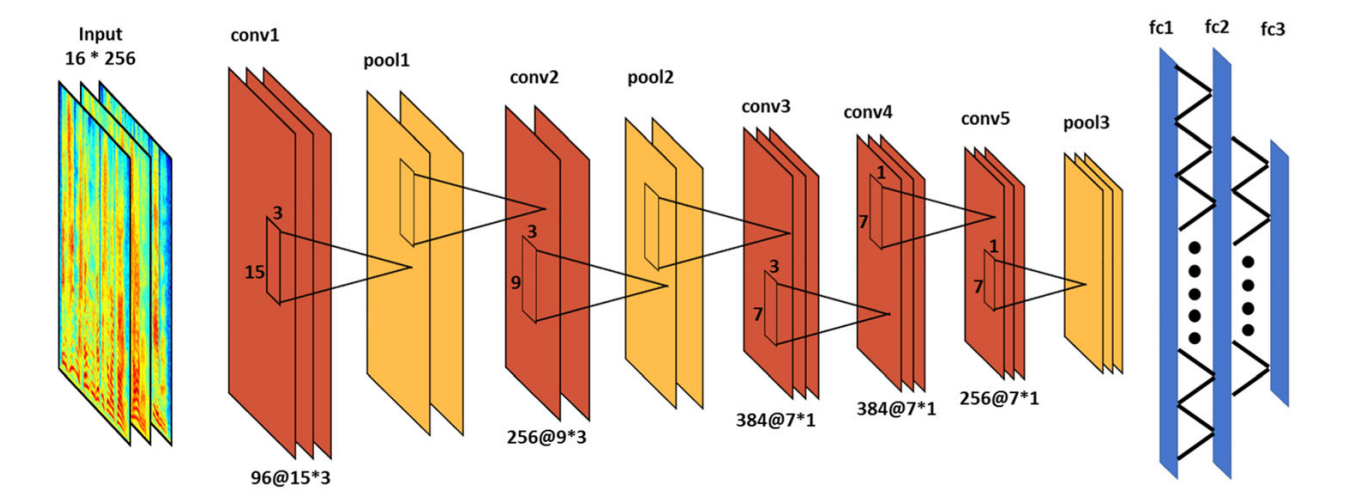
\includegraphics[width=1\textwidth]{images/conv}
    \caption{\label{architektur}CNN Architektur mit den unterschiedlichen Schichten \cite{badshah2019deep}}
\end{figure}

Mit Hilfe eines Labels kann man sich dann im Text auf diese Grafik (\ref{architektur}) beziehen. 



\section{Der Ablauf bei SER}

\begin{figure}[ht]
	\centering
	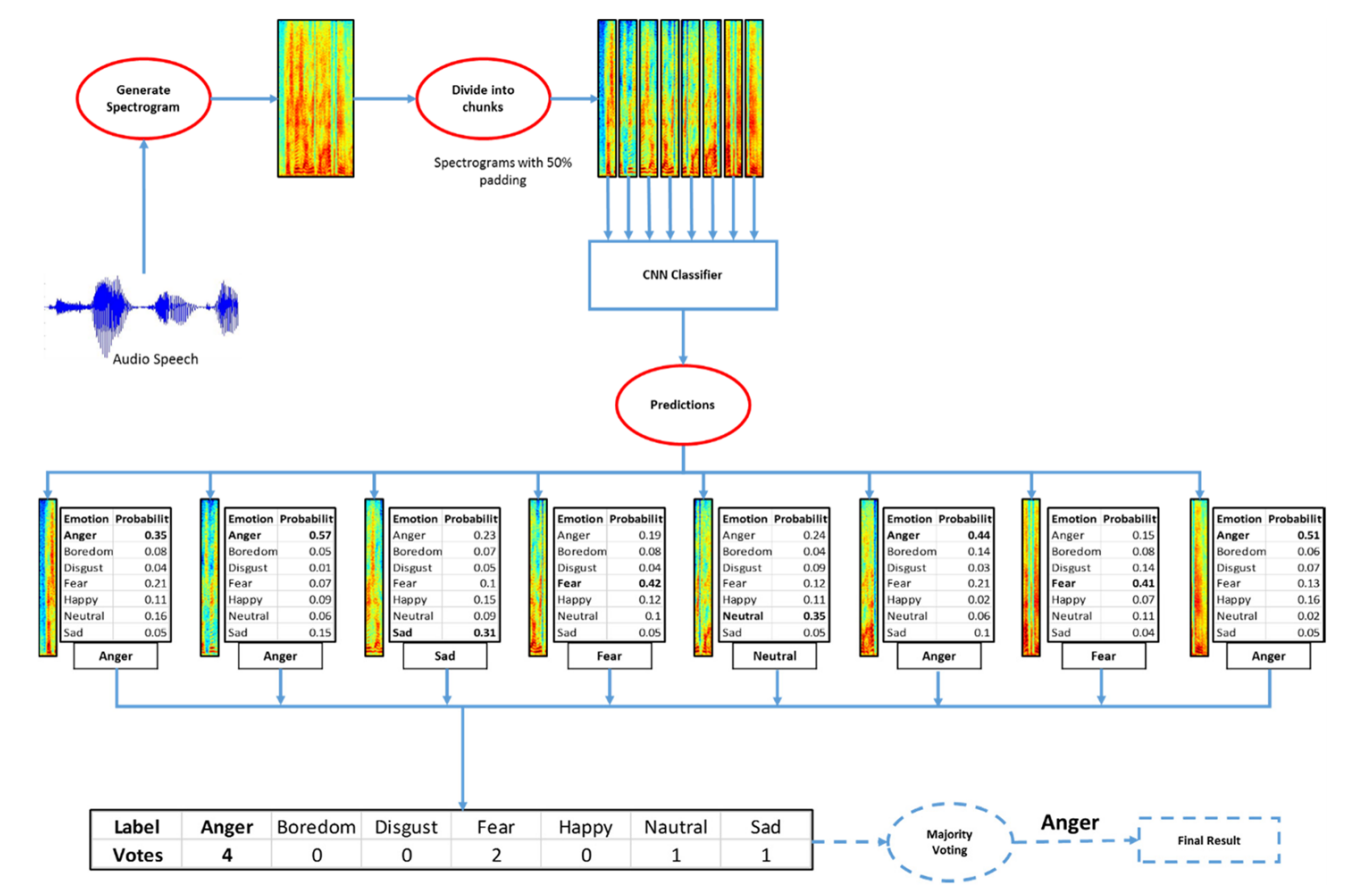
\includegraphics[width=1\textwidth]{images/ablauf}
	\caption{\label{ablauf}spezifischer Schema und Ablauf bei SER \cite{badshah2019deep}}
\end{figure}




